% Pursuing Stacks (cotes 134-2 to 134-8): archive cote 134-6, site page 30 (PDF page 31), typescript page 348.
% typescript. Draft compared: ps5.tex:2810-2882.
% AI-transcribed by Claude Opus 5.5 (claude-opus-5-5, adaptive thinking, effort high), Message Batches API, batch ps3 (msgbatch_01XdFmuVVBAcgc7EFxdtCqsj), 2026-11-12; reviewed against both supplied scan halves; see CHECK_DECISIONS.tsv.
\scanpage{134-6/30}
\mspage{348}

b)  Assume the contractibility structure $M_c$  non trivial,  i.e.
there exists an interval
\[ \underline{I} = (I,\hand{\delta}_0,\hand{\delta}_1) \quad \text{with} \quad I \hand{\in} M_c \ , \ \hand{\delta}_0 \neq \hand{\delta}_1 \ . \]
Then for any small category A and any functor
\[ i\colon A \hand{\longrightarrow} M \]
factoring through $M_c$ ,  the interval $i^*(\underline{I})$ in $A^\wedge$ is separating.  Hence
if  (for a given basic localizer $\underline{W}$) i is totally $\underline{W}$-aspheric (cf. theor\over{em}{em}
1 cor. 1  p.252),  hence $i^*(I)$ is totally aspheric in $A^\wedge$, \inserted{then} A is a \inserted[typed]{$\underline{W}$-}test
category.  In particular,  if A is totally $\underline{W}$-aspheric and i is
$M_a$-\inserted[typed]{$\underline{W}$-aspheric}\xout{\unsure{aspheric}},  A is a \inserted[typed]{strict $\underline{W}$-}\xout{local} test category.

\uline{Proof}   Part a) is a tautology in terms of section 51.  For part b),
to prove that $i^*(\underline{I})$ is separating,  we only have to check that for any
\xout{in $M_c$}  a in A ,  the two compositions
% Hand-drawn arrows are marked blue; typed objects remain plain.
\diagram{\begin{tikzcd} a \arrow[color=blue,r] & i^*(e_M) \hand{\simeq} e_{A^\wedge} \arrow[color=blue,r, shift left, "\hand{i^*(\delta_0),i^*(\delta_1)}"] \arrow[color=blue,r, shift right] & i^*(I) \end{tikzcd}}
are distinct,  or what amounts to the same by the definition of $i^*$ ,
that the compositions
% Hand-drawn arrows are marked blue; typed objects remain plain.
\diagram{\begin{tikzcd} i_{\hand{\unsure{!|*}}}(a) \overset{\mathrm{def}}{=} x \arrow[color=blue,r] & e_M \arrow[color=blue,r, shift left] \arrow[color=blue,r, shift right] & I \end{tikzcd}}
are \inserted[typed]{distinct}\xout{equal}.  As  x is in $M_c$ it has a sectio$\overset{\xout{\unsure{e}}}{\text{n}}$ over $e_M$ ,  so it is enough
to check that the compositions with  $e_M \hand{\longrightarrow} x$  are distinct,  which just
means that  $\hand{\delta}_0 \neq \hand{\delta}_1$  , qed.

\uline{Remark\over{s}{s}}\hand{.} \hand{1)} Part b) of the corollary replaces cor.3  on\hand{/}page 253,  which is
a little monster of incongruity (as I just discovered)  -  namely two
of the assumptions on $\underline{I}$  made there (namely that $\underline{I}$\xout{r} be a multiplicative
interval,  and $I \hand{\in} \mathrm{Ob}\, C$) are useless if we assume just I contractible,
moreover the \xout{assumptio} awkward separation assumption made there just
reduces by the \inserted[typed]{trivial} argument above to the assumption $\hand{\delta}_0 \neq \hand{\delta}_1$ !

\hand{2)} It should be noted that the \xout{contractibility s} homotopy structure
on $A^\wedge$ envisioned in th.1 \tikz[baseline=(ocue.base)]{\node[inner sep=0pt] (ocue) {o};\draw[color=blue] ([xshift=.3ex,yshift=.8ex]ocue.north) .. controls ([xshift=-.5ex]ocue.west) and ([xshift=-.2ex]ocue.south west) .. ([xshift=.2ex,yshift=-.2ex]ocue.south);}f section 79 (p.252)  is \uline{not} \deleted{thex} defined
as in the present section,  in terms of intervals in $A^\wedge$ coming from A
(call this structure h),  \uline{but as} 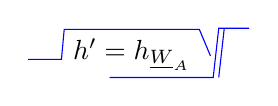
\begin{tikzpicture}[baseline=(fcue.base)]\node[inner sep=1pt] (fcue) {\ensuremath{h' = h_{\underline{W}_A}}};\draw[color=blue] ([xshift=-1.5em,yshift=-.4ex]fcue.west)--([xshift=-.3em,yshift=-.4ex]fcue.west)--([xshift=-.2em,yshift=.5ex]fcue.north west)--([xshift=.2em,yshift=.5ex]fcue.north east)--([xshift=.6em,yshift=-.1ex]fcue.east);\draw[color=blue] ([xshift=-.8em,yshift=-.3ex]fcue.south)--([xshift=.7em,yshift=-.3ex]fcue.south east)--([xshift=.9em,yshift=.6ex]fcue.north east)--([xshift=2em,yshift=.6ex]fcue.north east);\draw[color=blue] ([xshift=.9em,yshift=-.3ex]fcue.south east)--([xshift=1.1em,yshift=.6ex]fcue.north east);\end{tikzpicture} defined in terms of inter-% 
\margin{\tikz[baseline=(m.base)]{\node[inner sep=2pt] (m) {\shortstack{formule\\\`a la ligne}};\draw (m.center) ellipse (2.7em and 1.7em);}}
vals in $A^\wedge_{\mathrm{locas}}$\deleted{\illegible{1}} ; \inserted{this} \deleted{which} depends a priori on the choice of $\underline{W}$ ,  as it
has to because th.1  gives a criterion for the functor i to be $M_a$-$\underline{W}$-%
aspheric which does depend on $\underline{W}$ . (\over{i}{I}t surely wont be the same if we take
$\underline{W} = \underline{W}_\infty$  =  usual \inserted[typed]{weak} equivalence,  or $\underline{W} = F\mathord{\rlap{\text{/}}l}(\mathrm{Cat})$  hence $\underline{W}_A = F\mathord{\rlap{\text{/}}l}(A)$  and

\margin{30}

% Visual collation: both supplied image halves inspected; see CHECK_DECISIONS_134_7_8.tsv.
